\documentclass[12pt]{article}
\usepackage[utf8]{inputenc}
\usepackage[spanish, es-noshorthands]{babel}
\decimalpoint
\usepackage{amssymb,amsmath,amsthm,amsfonts,mathtools, bm}
\usepackage{tcolorbox}
\usepackage{microtype}

% ---- LINKS ----
\usepackage{hyperref}
\hypersetup{colorlinks=true, urlcolor=blue}

% ---- IMÁGENES ----
\usepackage{graphicx}
\graphicspath{ {imgs/} }

% ---- FORMATO DE TÍTULOS ----
\usepackage{titlesec}
\titlespacing{\section}{0pt}{1em plus 4pt minus 2pt}{0pt plus 2pt minus 2pt}
\titlespacing{\subsection}{0pt}{1em plus 4pt minus 2pt}{0pt plus 2pt minus 2pt}
\titlespacing{\subsubsection}{0pt}{1em plus 4pt minus 2pt}{0pt plus 2pt minus 2pt}

% ---- FORMATO DE LISTAS ----
\usepackage{enumitem}
\setlist[itemize]{topsep=-0.5em} % es media m para compensar
\setlist[enumerate]{topsep=-0.5em}

% ---- GRÁFICAS ----
\usepackage{tikz}
\usepackage{scalerel}
\usepackage{pict2e}
\usepackage{tkz-euclide}
\usetikzlibrary{calc}
\usetikzlibrary{patterns,arrows.meta}                   % Mejores flechas
\usetikzlibrary{shadows}                                % Sombras
\usetikzlibrary{external}                               % ¿?
\usetikzlibrary{decorations.pathreplacing,calligraphy}  % Para poder graficar el '{'
% Plots
\usepackage{pgfplots}
\pgfplotsset{compat=newest}                             % Ancho de las gráficas: width=6.5cm,
\usepgfplotslibrary{statistics}
\usepgfplotslibrary{fillbetween}

% ---- COLORES ----
\usepackage{xcolor}
\definecolor{miAzul}{RGB}{13, 33, 161}
\definecolor{miRojo}{RGB}{186, 24, 27}

% Para el pseudocódigo
\usepackage{algorithm}
\usepackage{algpseudocode}
\usepackage{amsmath}

\usepackage{listings}

% ---- FORMATO DE LAS PÁGINAS ----
\usepackage[a4paper, width=165mm, top=20mm, bottom = 20mm]{geometry}
\usepackage{fancyhdr}
\pagestyle{fancy}
% Primera página. Comentar si se quiere que todas sean iguales
\fancypagestyle{firststyle}{
   \fancyhf{}
   \fancyfoot[R]{\footnotesize \thepage}
   \renewcommand{\headrulewidth}{0pt}
}
% Para el resto del documento.
\fancyhf{}
\lhead{\footnotesize Formulación y solución de P.P.L.}
\chead{\footnotesize \textbf{Proyecto final}}
\rhead{\footnotesize \today}
\lfoot{\footnotesize Equipo 4}
\cfoot{\footnotesize \textsc{Programación Lineal}}
\rfoot{\footnotesize \thepage}

\renewcommand{\headrulewidth}{0.4pt}
\renewcommand{\footrulewidth}{0.4pt}
\setlength{\headheight}{15pt}

\setlength{\parskip}{1em}
\setlength{\parindent}{0cm}

% ---- TEXTO DE RELLENO ----
\usepackage{lipsum}  

\title{
    La Materia \\
    \large Título
}
\author{José Alberto Márquez Luján, 187917}
\date{\today}

\begin{document}
\begin{titlepage}
	\centering
	
\includegraphics[width=0.5\textwidth]{logo-ITAM.pdf}\par\vspace{1cm}
	{\scshape\large Instituto Tecnológico Autónomo de México \par}
	\vspace{2.5cm}
	
	{\scshape\Large Programación Lineal\par}
	\vspace{1.5cm}
	{\LARGE\bfseries Proyecto final\par}
    \vspace{0.5cm}
	{\large\bfseries Formulación y solución de problemas de programación lineal}
	\vspace{3cm}
	
	{\large
	\begin{tabular}{||l c||} 
         \hline
         \multicolumn{1}{||c}{\textbf{Integrantes del equipo}} & \textbf{Clave única} \\
         \hline\hline
         Karen Arteaga Mendoza & \texttt{190161} \\ 
         \hline
         Federico Santacruz González & \texttt{190438}\\
         \hline
         Leopoldo Rodríguez Díaz Infante & \texttt{189584} \\ 
         \hline
         José Alberto Márquez Luján & \texttt{187917} \\
         \hline
         Santiago Fernández del Castillo Sodi & \texttt{189210} \\
         \hline
    \end{tabular}
    }
	\vfill
	Profesor:\par
	Dr.~Edgar Possani Espinosa

	\vfill
	{\today\par}
\end{titlepage}

\section{Reporte técnico - Caso 4.2}
Para formular el problema de programación lineal en su forma estándar, pensemos que tenemos lo siguiente:
\begin{figure}[ht]
    \centering
    \begin{tabular}{|l|c|c|c|c|}
     \hline
     \textbf{Entrevistados} & 18-25 & 26-40 & 41-50 & 51+ \\
     \hline 
     Silicon Valley & $x_1$ & $x_2$    & $x_3$    & $x_4$ \\
     Big cities     & $x_5$ & $x_6$    & $x_7$    & $x_8$ \\
     Small towns    & $x_9$ & $x_{10}$ & $x_{11}$ & $x_{12}$ \\
     \hline 
    \end{tabular}    
    \label{fig:tabla1}
\end{figure}

Así, podemos construir al vector $\pmb{x} = (x_1, \ldots, x_{12})$ con las variables de decisión del problema. Cada entrada $x_i$ representa la cantidad de personas entrevistadas pertenecientes a un determinado grupo de edad y región. Análogamente tenemos al vector de costos $\pmb{c}^T = (c_1, \ldots, c_{12})$, en donde cada entrada está dada por el costo que tiene entrevistar a la persona asociada al mismo grupo de edad y región.
\begin{figure}[ht]
    \centering
    \begin{tabular}{|l|c|c|c|c|}
     \hline
     \textbf{Costos} & 18-25 & 26-40 & 41-50 & 51+ \\
     \hline 
     Silicon Valley & $c_1$ & $c_2$    & $c_3$    & $c_4$ \\
     Big cities     & $c_5$ & $c_6$    & $c_7$    & $c_8$ \\
     Small towns    & $c_9$ & $c_{10}$ & $c_{11}$ & $c_{12}$ \\
     \hline 
    \end{tabular}    
    \label{fig:tabla2}
\end{figure}

Nótese que 
\[ \pmb{c}^T \cdot \pmb{x} = \sum_{i=1}^{12}c_i x_i \]
nos da el costo total que tendría Sophisticated Surveys por realizar la encuesta. Nos interesa minimizar este valor. El margen de la empresa Sophisticated Surveys no es de interés en este momento. Ahora bien, Rob nos impone ciertas restricciones. Para empezar, es necesario que la suma de los entrevistados sea exactamente $2000$; esto es, 
\[ \sum_{i=1}^n x_i = 2000. \]
Además, hay ciertos porcentajes que hay que cumplir:
\begin{figure}[ht]
    \centering
    \begin{tabular}{|c|c|c|}
     \hline
     \textbf{Grupo de edad} & \textbf{Porcentaje mínimo} & \textbf{Cantidad mínima} \\
     \hline 
     18-25 & 20.0\%   & 400 \\
     26-40 & 27.5\%   & 550 \\
     41-50 & 15.0\%   & 300 \\
     51+   & 15.0\%   & 300 \\
     \hline 
    \end{tabular}    
    \label{fig:tabla3}
\end{figure}

Así pues, tenemos otras cuatro restricciones:
\begin{align*}
    x_1 + x_5 + x_9 &\geq 400 \\
    x_2 + x_6 + x_{10} &\geq 350 \\
    x_3 + x_7 + x_{11} &\geq 300 \\
    x_4 + x_8 + x_{12} &\geq 300 \\
\end{align*}

En adición a estas restricciones, sabemos que Rob quiere que la encuesta cumpla ciertos requisitos sobre las regiones en las que se va a entrevistar, como podemos ver en la tabla (\ref{fig:tabla4}).
\begin{figure}[ht]
    \centering
    \begin{tabular}{|c|c|c|}
     \hline
     \textbf{Región} & \textbf{Porcentaje mínimo} & \textbf{Cantidad mínima} \\
     \hline 
     Silicon Valley & 15.0\%   & 300 \\
     Big cities     & 35.0\%   & 700 \\
     Small towns    & 20.0\%   & 400 \\     
     \hline 
    \end{tabular}    
    \label{fig:tabla4}
\end{figure}

Esto nos impone otras tres restricciones:
\begin{align*}
    x_1 + x_2 + x_3 + x_4 &\geq 300 \\
    x_5 + x_6 + x_7 + x_8 &\geq 700 \\
    x_9 + x_{10} + x_{11} + x_{12} &\geq 400 
\end{align*}

Hasta ahora todas las restricciones, a excepción de la primera, son de la forma ``es mayor o igual que''; sin embargo, a nosotros nos interesa que las restricciones sean del tipo ``es igual a''. Para ello, agregamos variables de excedente a cada una de las 7 restricciones:
\begin{align*}
    x_1 + x_5 + x_9 - e_1&= 400 \\
    x_2 + x_6 + x_{10} - e_2&= 350 \\
    x_3 + x_7 + x_{11} - e_3&= 300 \\
    x_4 + x_8 + x_{12} - e_4&= 300 \\
    x_1 + x_2 + x_3 + x_4 - e_5&= 300 \\
    x_5 + x_6 + x_7 + x_8 - e_6&= 700 \\
    x_9 + x_{10} + x_{11} + x_{12} - e_7&= 400 
\end{align*}
donde $e_i \geq 0$ para toda $i \in \{1, \ldots, 7\}$. Como $x_i$ denota al número de personas entrevistadas, entonces es natural suponer que $x_i \geq 0$ para cualquier $i \in \{1, \ldots, 12\}$. Así, pues, el problema de programación lineal en su forma estándar nos queda:

\[ \min \biggl\{ z = \sum_{i=1}^{12} c_i x_{i} \biggr\} \]
sujeto a
\begin{align*}
    \sum_{i=1}^{12} x_i &= 2000 \\
    x_1 + x_5 + x_9 - e_1&= 400 \\
    x_2 + x_6 + x_{10} - e_2&= 350 \\
    x_3 + x_7 + x_{11} - e_3&= 300 \\
    x_4 + x_8 + x_{12} - e_4&= 300 \\
    x_1 + x_2 + x_3 + x_4 - e_5&= 300 \\
    x_5 + x_6 + x_7 + x_8 - e_6&= 700 \\
    x_9 + x_{10} + x_{11} + x_{12} - e_7&= 400    
\end{align*}
\[ x_i, e_j \geq 0 \quad \forall i \in \{1,\ldots,12\}, j \in \{1,\ldots,7\}. \]

Si queremos expresar el problema en su forma matricial, como ahora hemos agregado variables de excedente, tenemos que incrementar el tamaño de nuestros vectores $\pmb{x}$ y $\pmb{c}^T$. Al primero hay que agregarle las variables de excedente como tal y al segundo asociarle costos de cero a cada variable de excedente, pues no nos importa el valor de dichas variables para el problema planteado. Entonces $\pmb{x} = (x_1, \ldots, x_{12}, e_1, \ldots, e_7)$ y $\pmb{c}^T = (c_1, \ldots, c_{12}, 0, \ldots, 0)$.

La matriz $A$ estaría dada por
\begin{figure}[ht]
    \centering
    \begin{tabular}{lllllllllllllllllll}
        $x_1$ & $x_2$ & $x_3$ & $x_4$ & $x_5$ & $x_6$ & $x_7$ & $x_8$ & $x_9$ & $x_{10}$ & $x_{11}$ & $x_{12}$ & $e_1$ & $e_2$ & $e_3$ & $e_4$ & $e_5$ & $e_6$ & $e_7$ \\
        1   & 1   & 1   & 1   & 1   & 1   & 1   & 1   & 1   & 1      & 1      & 1      & 0   & 0   & 0   & 0   & 0   & 0   & 0   \\
        1   & 0   & 0   & 0   & 1   & 0   & 0   & 0   & 1   & 0      & 0      & 0      & -1  & 0   & 0   & 0   & 0   & 0   & 0   \\
        0   & 1   & 0   & 0   & 0   & 1   & 0   & 0   & 0   & 1      & 0      & 0      & 0   & -1  & 0   & 0   & 0   & 0   & 0   \\
        0   & 0   & 1   & 0   & 0   & 0   & 1   & 0   & 0   & 0      & 1      & 0      & 0   & 0   & -1  & 0   & 0   & 0   & 0   \\
        0   & 0   & 0   & 1   & 0   & 0   & 0   & 1   & 0   & 0      & 0      & 1      & 0   & 0   & 0   & -1  & 0   & 0   & 0   \\
        1   & 1   & 1   & 1   & 0   & 0   & 0   & 0   & 0   & 0      & 0      & 0      & 0   & 0   & 0   & 0   & -1  & 0   & 0   \\
        0   & 0   & 0   & 0   & 1   & 1   & 1   & 1   & 0   & 0      & 0      & 0      & 0   & 0   & 0   & 0   & 0   & -1  & 0   \\
        0   & 0   & 0   & 0   & 0   & 0   & 0   & 0   & 1   & 1      & 1      & 1      & 0   & 0   & 0   & 0   & 0   & 0   & -1 
        \end{tabular}
    \label{fig:tabla5}
\end{figure}

y el vector $\pmb{b} = (2000, 400, 350, 300, 300, 300, 700, 400)$.

Así pues, el problema sería minimizar $z = \pmb{c}^T \cdot \pmb{x}$ sujeto a $A \pmb{x} = b$, con $\pmb{x} \geq 0$.

La solución al planteamiento inicial se muestra en la figura (\ref{fig:img1}).
\begin{figure}
    \centering
    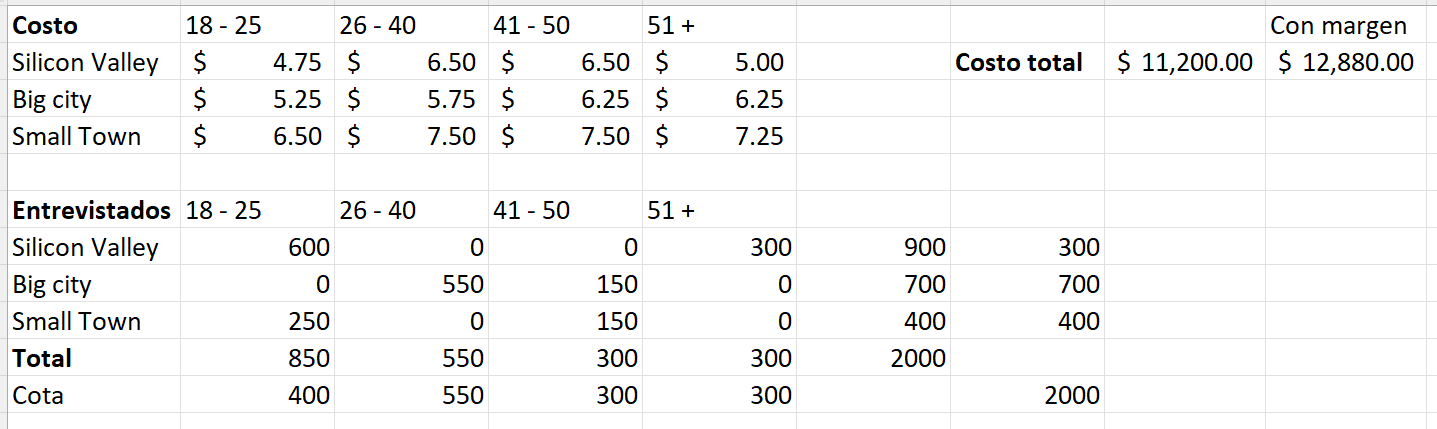
\includegraphics[scale=0.4]{imgs/inicial.png} 
    \caption{Situación inicial.}
    \label{fig:img1}   
\end{figure}

Si la muestra de población inicial no es lo suficientemente representativa y hay que agregar una restricción en la cual debe de haber, por lo menos, 50 personas de cada grupo de edad, entonces se agrega la restricción de que $x_i \geq 0$ para toda $i \in \{1,\ldots,12\}$. El ajuste correspondiente se muestra en la figura (\ref{fig:img2}).
\begin{figure}
    \centering
    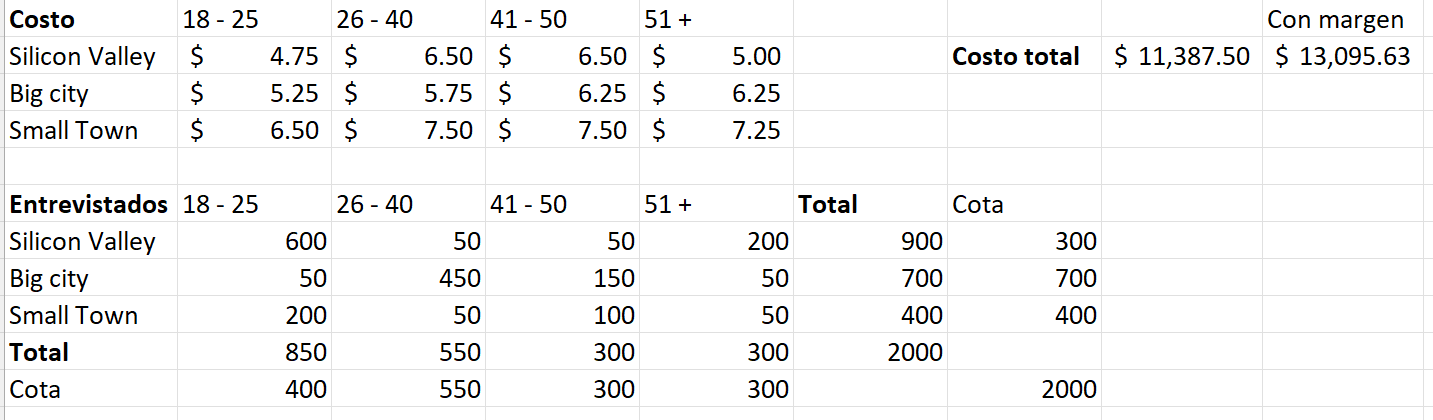
\includegraphics[scale=0.4]{imgs/ajuste1.png}
    \caption{Primer ajuste.}    
    \label{fig:img2}   
\end{figure}

Considerando que hay un exceso de muestras para la población de 18-25 años y la de Silicon Valley, y que Rob exige un máximo de 600 y 650 individuos respectivamente, se agregan dos restricciones más:
\begin{align*}
    x_1 + x_2 + x_9 &\leq 600 \\
    x_1 + x_2 + x_3 + x_4 &\leq 650
\end{align*}
El ajuste correspondiente se muestra en la figura (\ref{fig:img3}).
\begin{figure}
    \centering
    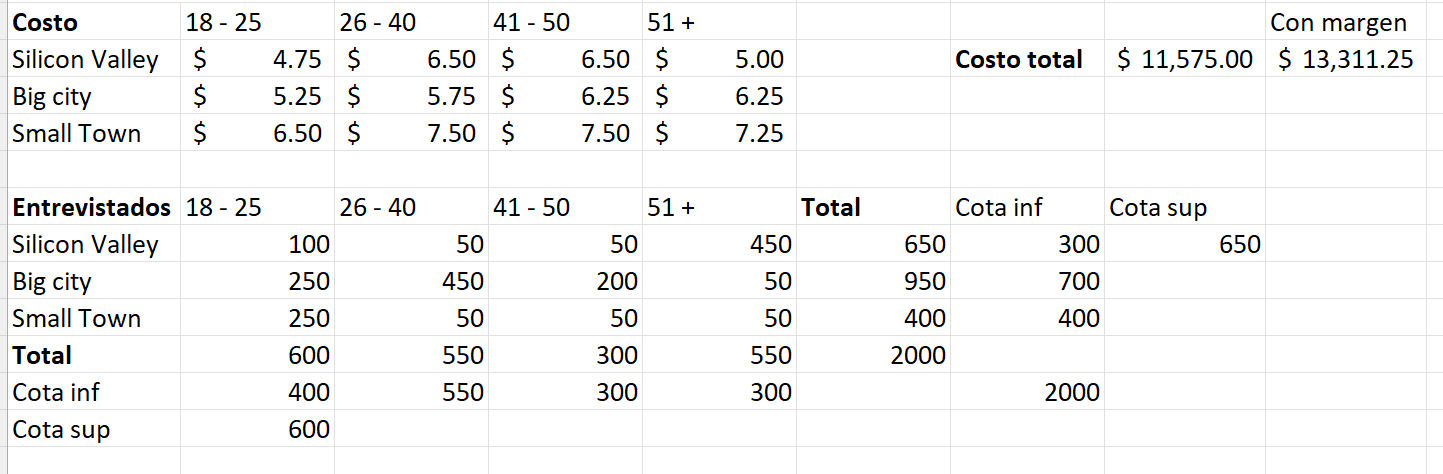
\includegraphics[scale=0.4]{imgs/ajuste2.png}
    \caption{Segundo ajuste.}    
    \label{fig:img3}   
\end{figure}

El siguiente ajuste exige que cambien los costos; esto es, nuestro vector $\pmb{c}^T$. Ahora $c_1 = 6.5, c_5 = 6.75$ y $c_9 = 7$. El ajuste correspondiente se muestra en la figura (\ref{fig:img4}).
\begin{figure}
    \centering
    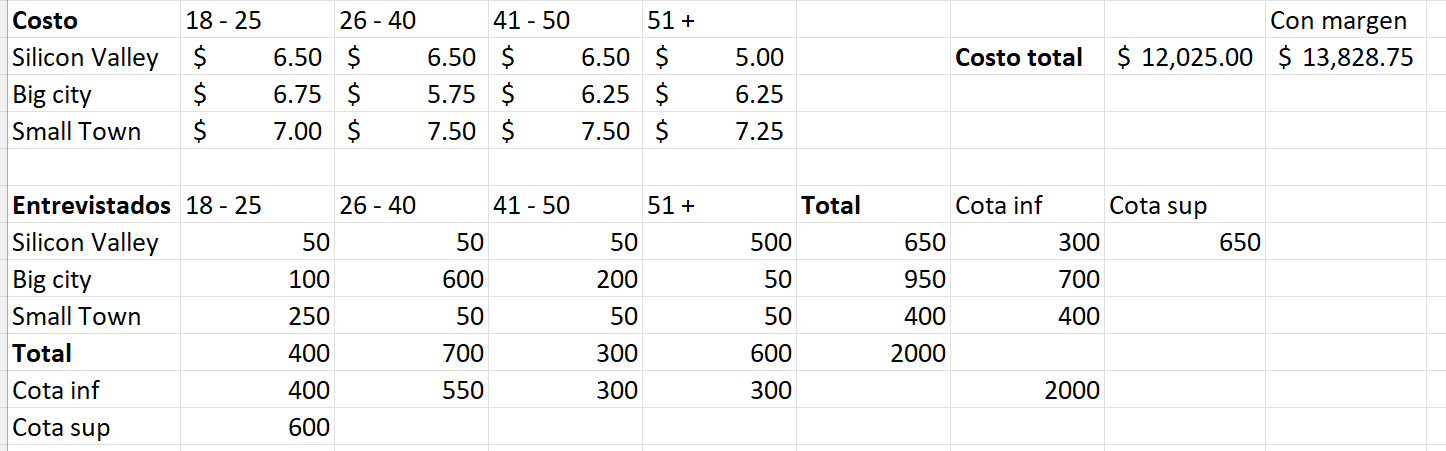
\includegraphics[scale=0.4]{imgs/ajuste3.png}
    \caption{Tercer ajuste.}    
    \label{fig:img4}   
\end{figure}

Finalmente, ante los requisitos más estrictos que solicitó Rob al fijar los porcentajes de gente encuestada para cada población, tenemos que eliminar nuestras variables de excedente (las $e_i$'s) y cambiar el vector $\pmb{b}$ de manera que se cumpla lo que Rob solicita. El ajuste correspondiente se muestra en la figura (\ref{fig:img5}).
\begin{figure}
    \centering
    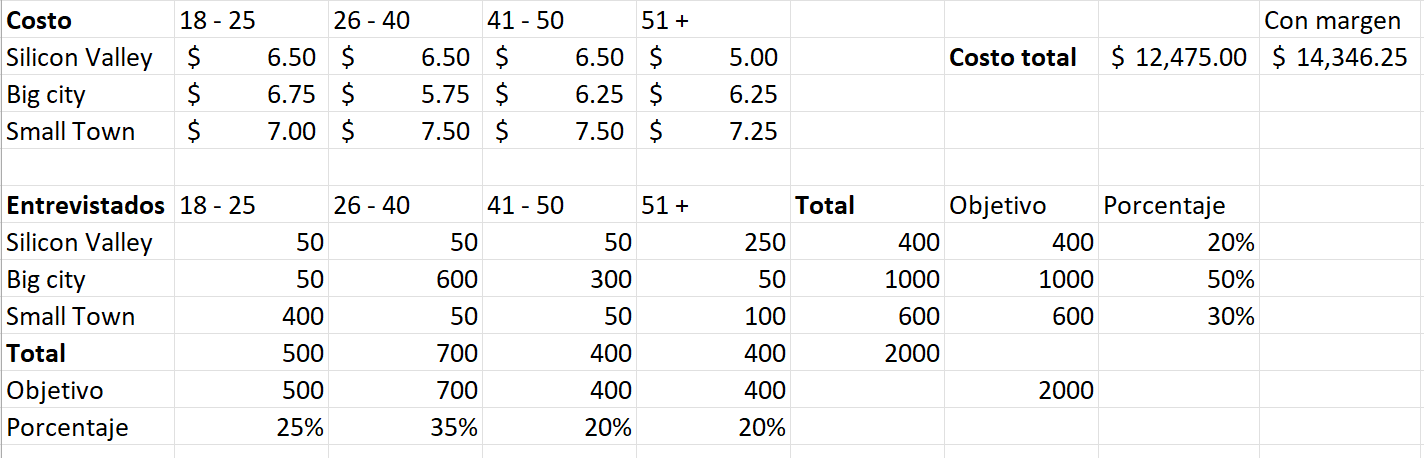
\includegraphics[scale=0.4]{imgs/ajuste4.png}
    \caption{Cuarto ajuste.}    
    \label{fig:img5}   
\end{figure}

%%%%%% FIN DEL TEXTO %%%%%%

\end{document}